\documentclass[11pt]{article}
% Print layout. The editable article and its captions are in article.tex.
\usepackage[utf8]{inputenc}
\usepackage[T1]{fontenc}
\usepackage{lmodern,charter}
\usepackage[a4paper,left=.8in,right=.8in,top=.65in,bottom=.7in,footskip=.35in]{geometry}
\usepackage{graphicx,xcolor,caption,float,fancyhdr,titlesec}
\usepackage{hyperref}
\definecolor{Ink}{HTML}{152E3E}
\definecolor{Copper}{HTML}{9D4D24}
\definecolor{Secondary}{HTML}{475E68}
\hypersetup{colorlinks=true,urlcolor=Copper,linkcolor=Ink,pdftitle={Seven Green Tests. One Broken Fix.},pdfauthor={Enrico Papalini}}
\setlength{\parindent}{0pt}
\setlength{\parskip}{5pt plus .3pt minus .3pt}
\setlength{\intextsep}{10pt}
\renewcommand{\baselinestretch}{1.06}
\emergencystretch=1.5em
\raggedbottom
\frenchspacing
\setcounter{secnumdepth}{0}
\titleformat{\section}{\sffamily\bfseries\color{Ink}\fontsize{17}{20}\selectfont}{}{0pt}{}
\titlespacing*{\section}{0pt}{13pt plus 1pt}{6pt}
\captionsetup{labelformat=empty,justification=raggedright,singlelinecheck=false,font={sf,small,color=Secondary},skip=5pt}
\pagestyle{fancy}
\fancyhf{}
\renewcommand{\headrulewidth}{0pt}
\renewcommand{\footrulewidth}{.25pt}
\fancyfoot[L]{\sffamily\footnotesize\color{Secondary}Enrico Papalini\enspace/\enspace The Non-Deterministic series}
\fancyfoot[R]{\sffamily\footnotesize\color{Secondary}\thepage}
\makeatletter
\renewcommand{\maketitle}{\noindent{\raggedright\rightskip=.17\linewidth plus 1fil\sffamily\bfseries\fontsize{30}{34}\selectfont\color{Ink}\@title\par}}
\renewenvironment{abstract}{\par\begingroup\sffamily\large\color{Secondary}\setlength{\parskip}{0pt}}{\par\endgroup\vspace{5pt}{\sffamily\small\bfseries\color{Copper}\@author\par}\vspace{5pt}}
\makeatother

\title{Seven Green Tests. One Broken Fix.}
\author{Enrico Papalini}
\date{}
\begin{document}
\maketitle
\begin{abstract}
A negative cent reveals what engineers must still own when AI writes the code.
\end{abstract}

All seven tests pass. The repaired function still sends \texttt{Infinity} to human review.

That is a deliberately incomplete repair in the opening chapter of \emph{Engineering Software with Agentic AI}. It exposes a question every engineer delegating work to an agent needs to answer: \textbf{what, exactly, does the evidence allow me to accept?}

The book's Treasury teaching case begins with EUR~-0.01 reaching the standard queue. Operations must investigate a request the software should have rejected. This system selects a queue; payment authorisation lies outside its scope.

The faulty function looks straightforward. Parse the amount, compare it with EUR~5,000, choose a queue. A negative number is below 5,000, so it takes the ordinary route.

I begin the book here because a small repair makes the engineer's decisions visible: the approved rule, the agent's work and the observations behind the acceptance decision.

\section{Write down the answer before asking for the fix}

The approved rule, BR-001/v1, requires a parseable decimal that is finite and strictly positive. Invalid amounts are rejected. Valid amounts below EUR~5,000 enter the standard queue; EUR~5,000 and above require human review. Every result identifies the policy version used.

Before inspecting the implementation, write down three expectations: reject \texttt{-0.01}, keep \texttt{4000.00} in the standard queue, and send \texttt{5000.00} to human review.

That last expectation already works in the starter. The repair must preserve it.

\begin{figure}[H]
\centering
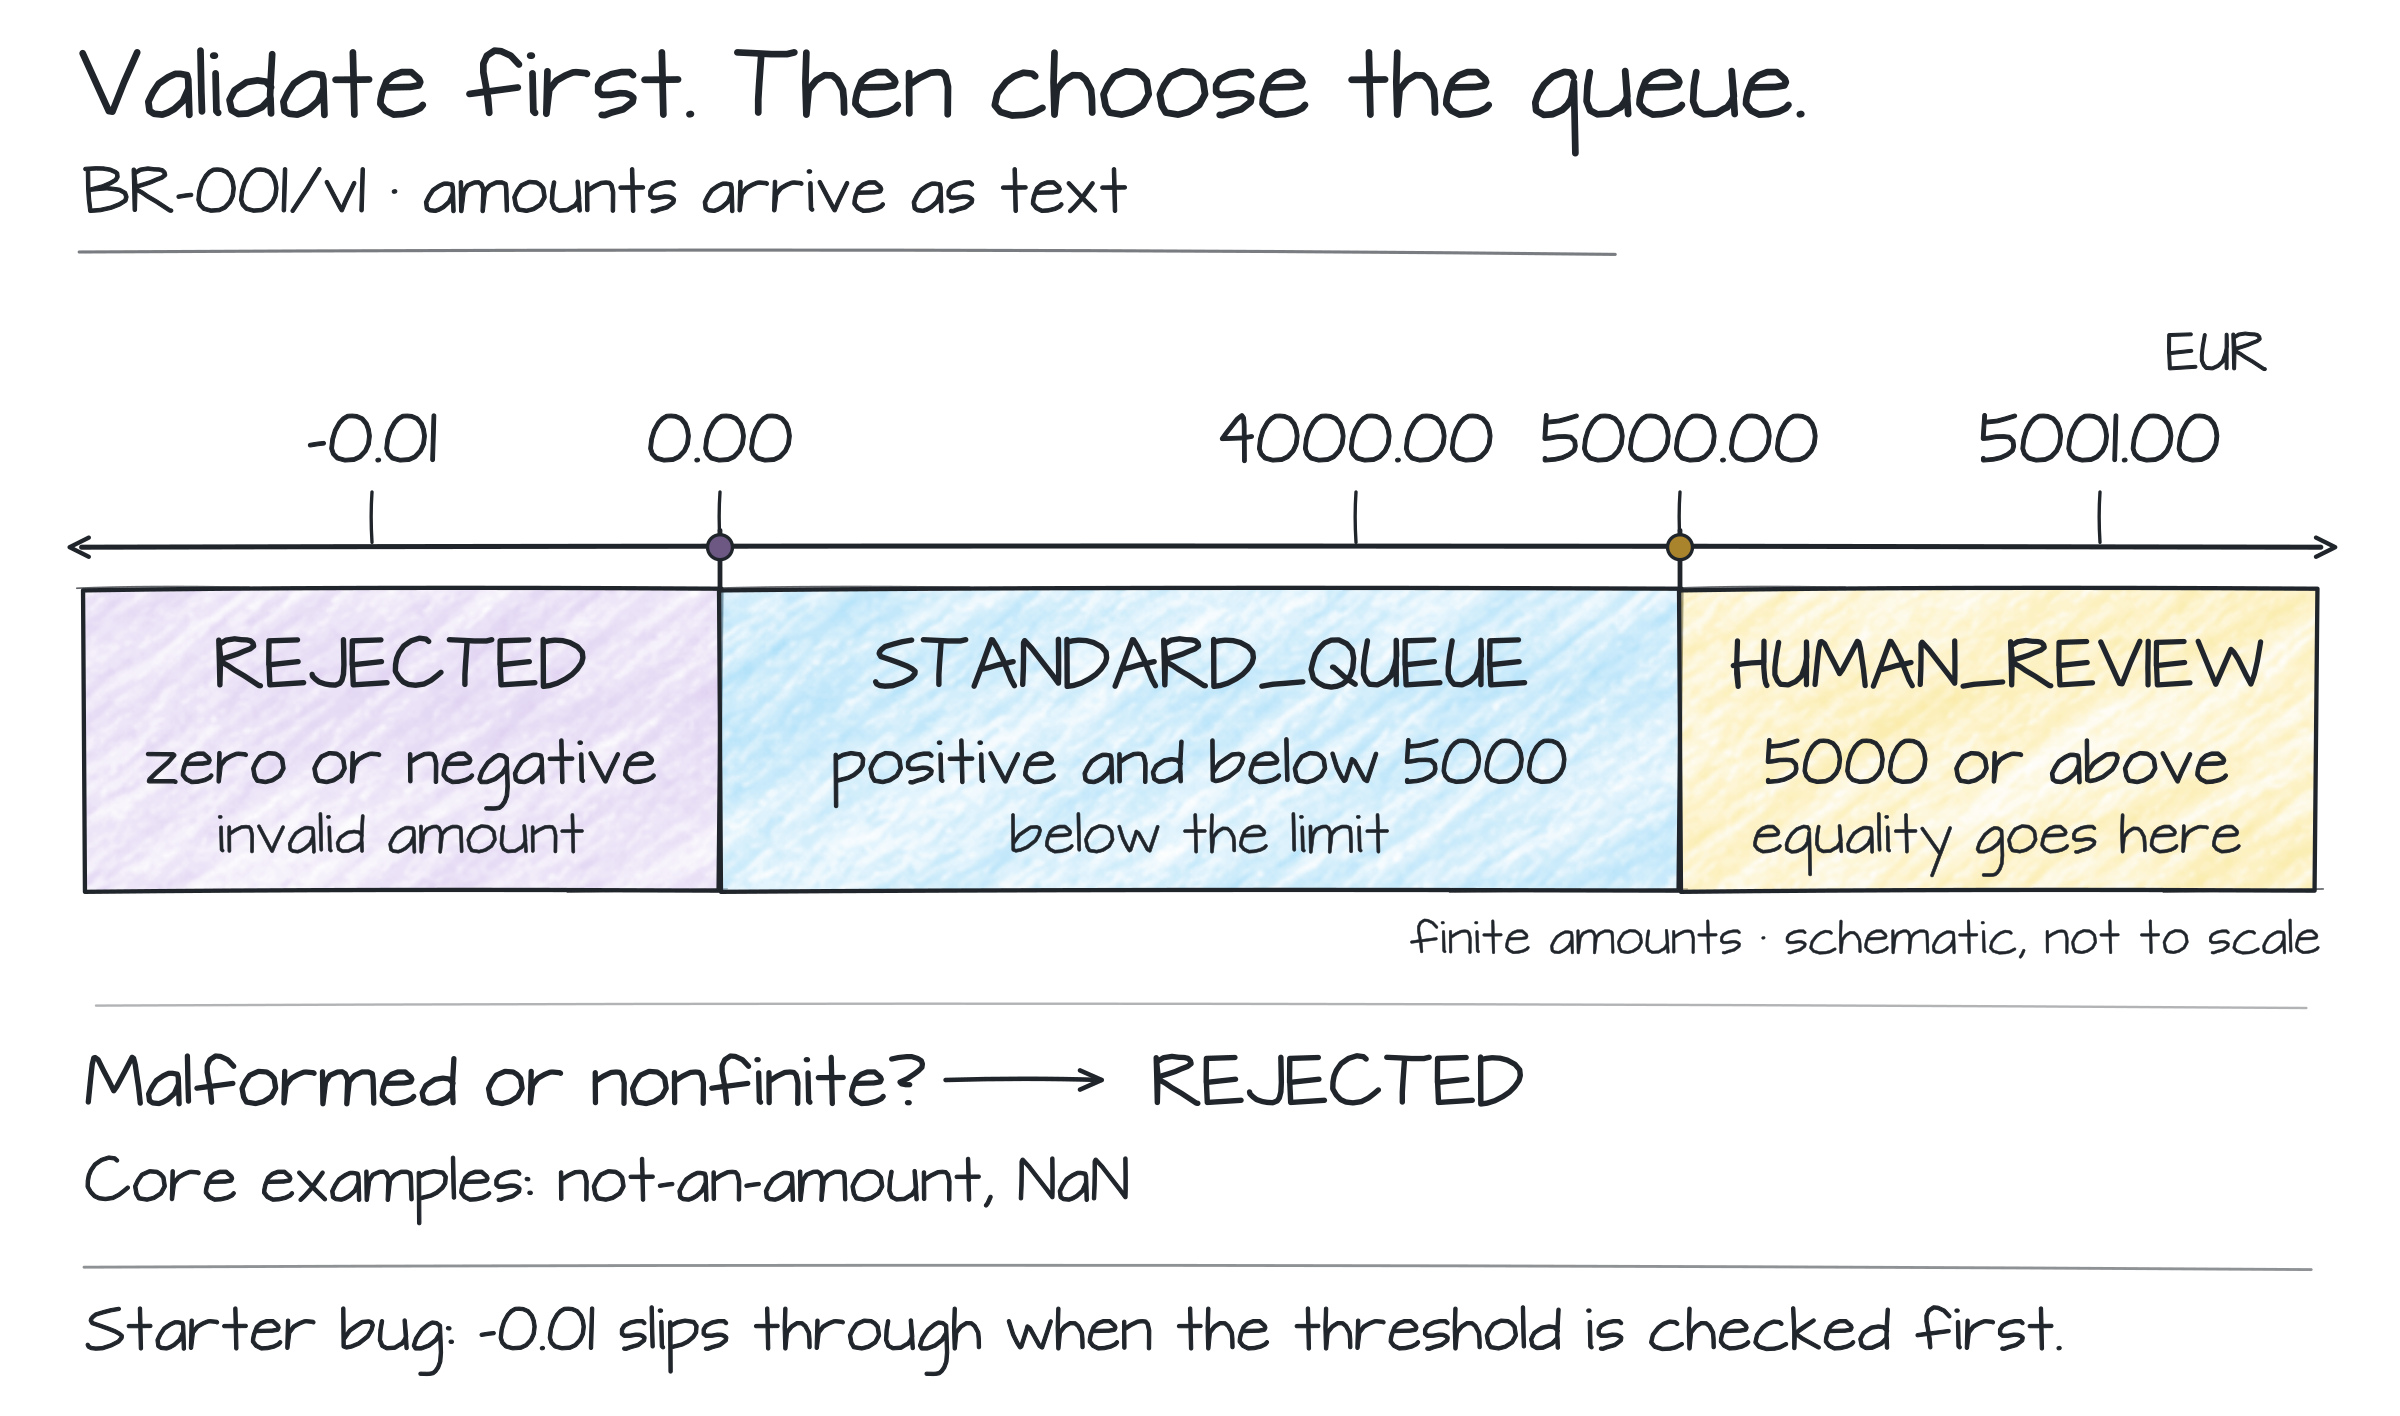
\includegraphics[width=.95\linewidth]{assets/boundaries.jpg}
\caption{The approved rule determines the answer. Validate the amount before comparing it with the threshold. Hand-drawn adaptation of Figure~1.2 in Chapter~1.}
\end{figure}

\clearpage
\section{The baseline tells you what to protect}

Run the seven core cases on the unchanged starter. Three pass: below, at and above the threshold. Negative and zero amounts take the wrong route; malformed text and \texttt{NaN} raise errors.

Those outcomes describe different obligations. A positivity guard addresses negative and zero values. Parsing failures and nonfinite values still need attention. The three existing passes identify behaviour the change must preserve.

Now the agent's task can be specific: repair invalid-amount handling while retaining the interface, policy identity and EUR~5,000 boundary. Edit the router. Keep the governing documents and acceptance checks protected. Stop when the work requires an unresolved policy decision.

That boundary matters. The agent can physically edit a threshold without having authority to change it. A newer-looking note proposing EUR~10,000 does not acquire approval merely by appearing in the repository.

\section{Give the agent a bounded job}

The chapter organises this work into four responsibilities: \textbf{Expect, Delegate, Observe, Decide}, or EDOD.

Expect establishes the authorised outcome and examples. Delegate states what the agent may change, what it must preserve and when to stop. Observe independently checks the actual candidate against controlled expectations. Decide names the result the accountable reviewer can accept, reject or refer to an owner.

One engineer can perform several of these jobs. Keeping the responsibilities explicit lets us examine where an expectation came from and which change an observation actually covers.

\begin{figure}[H]
\centering
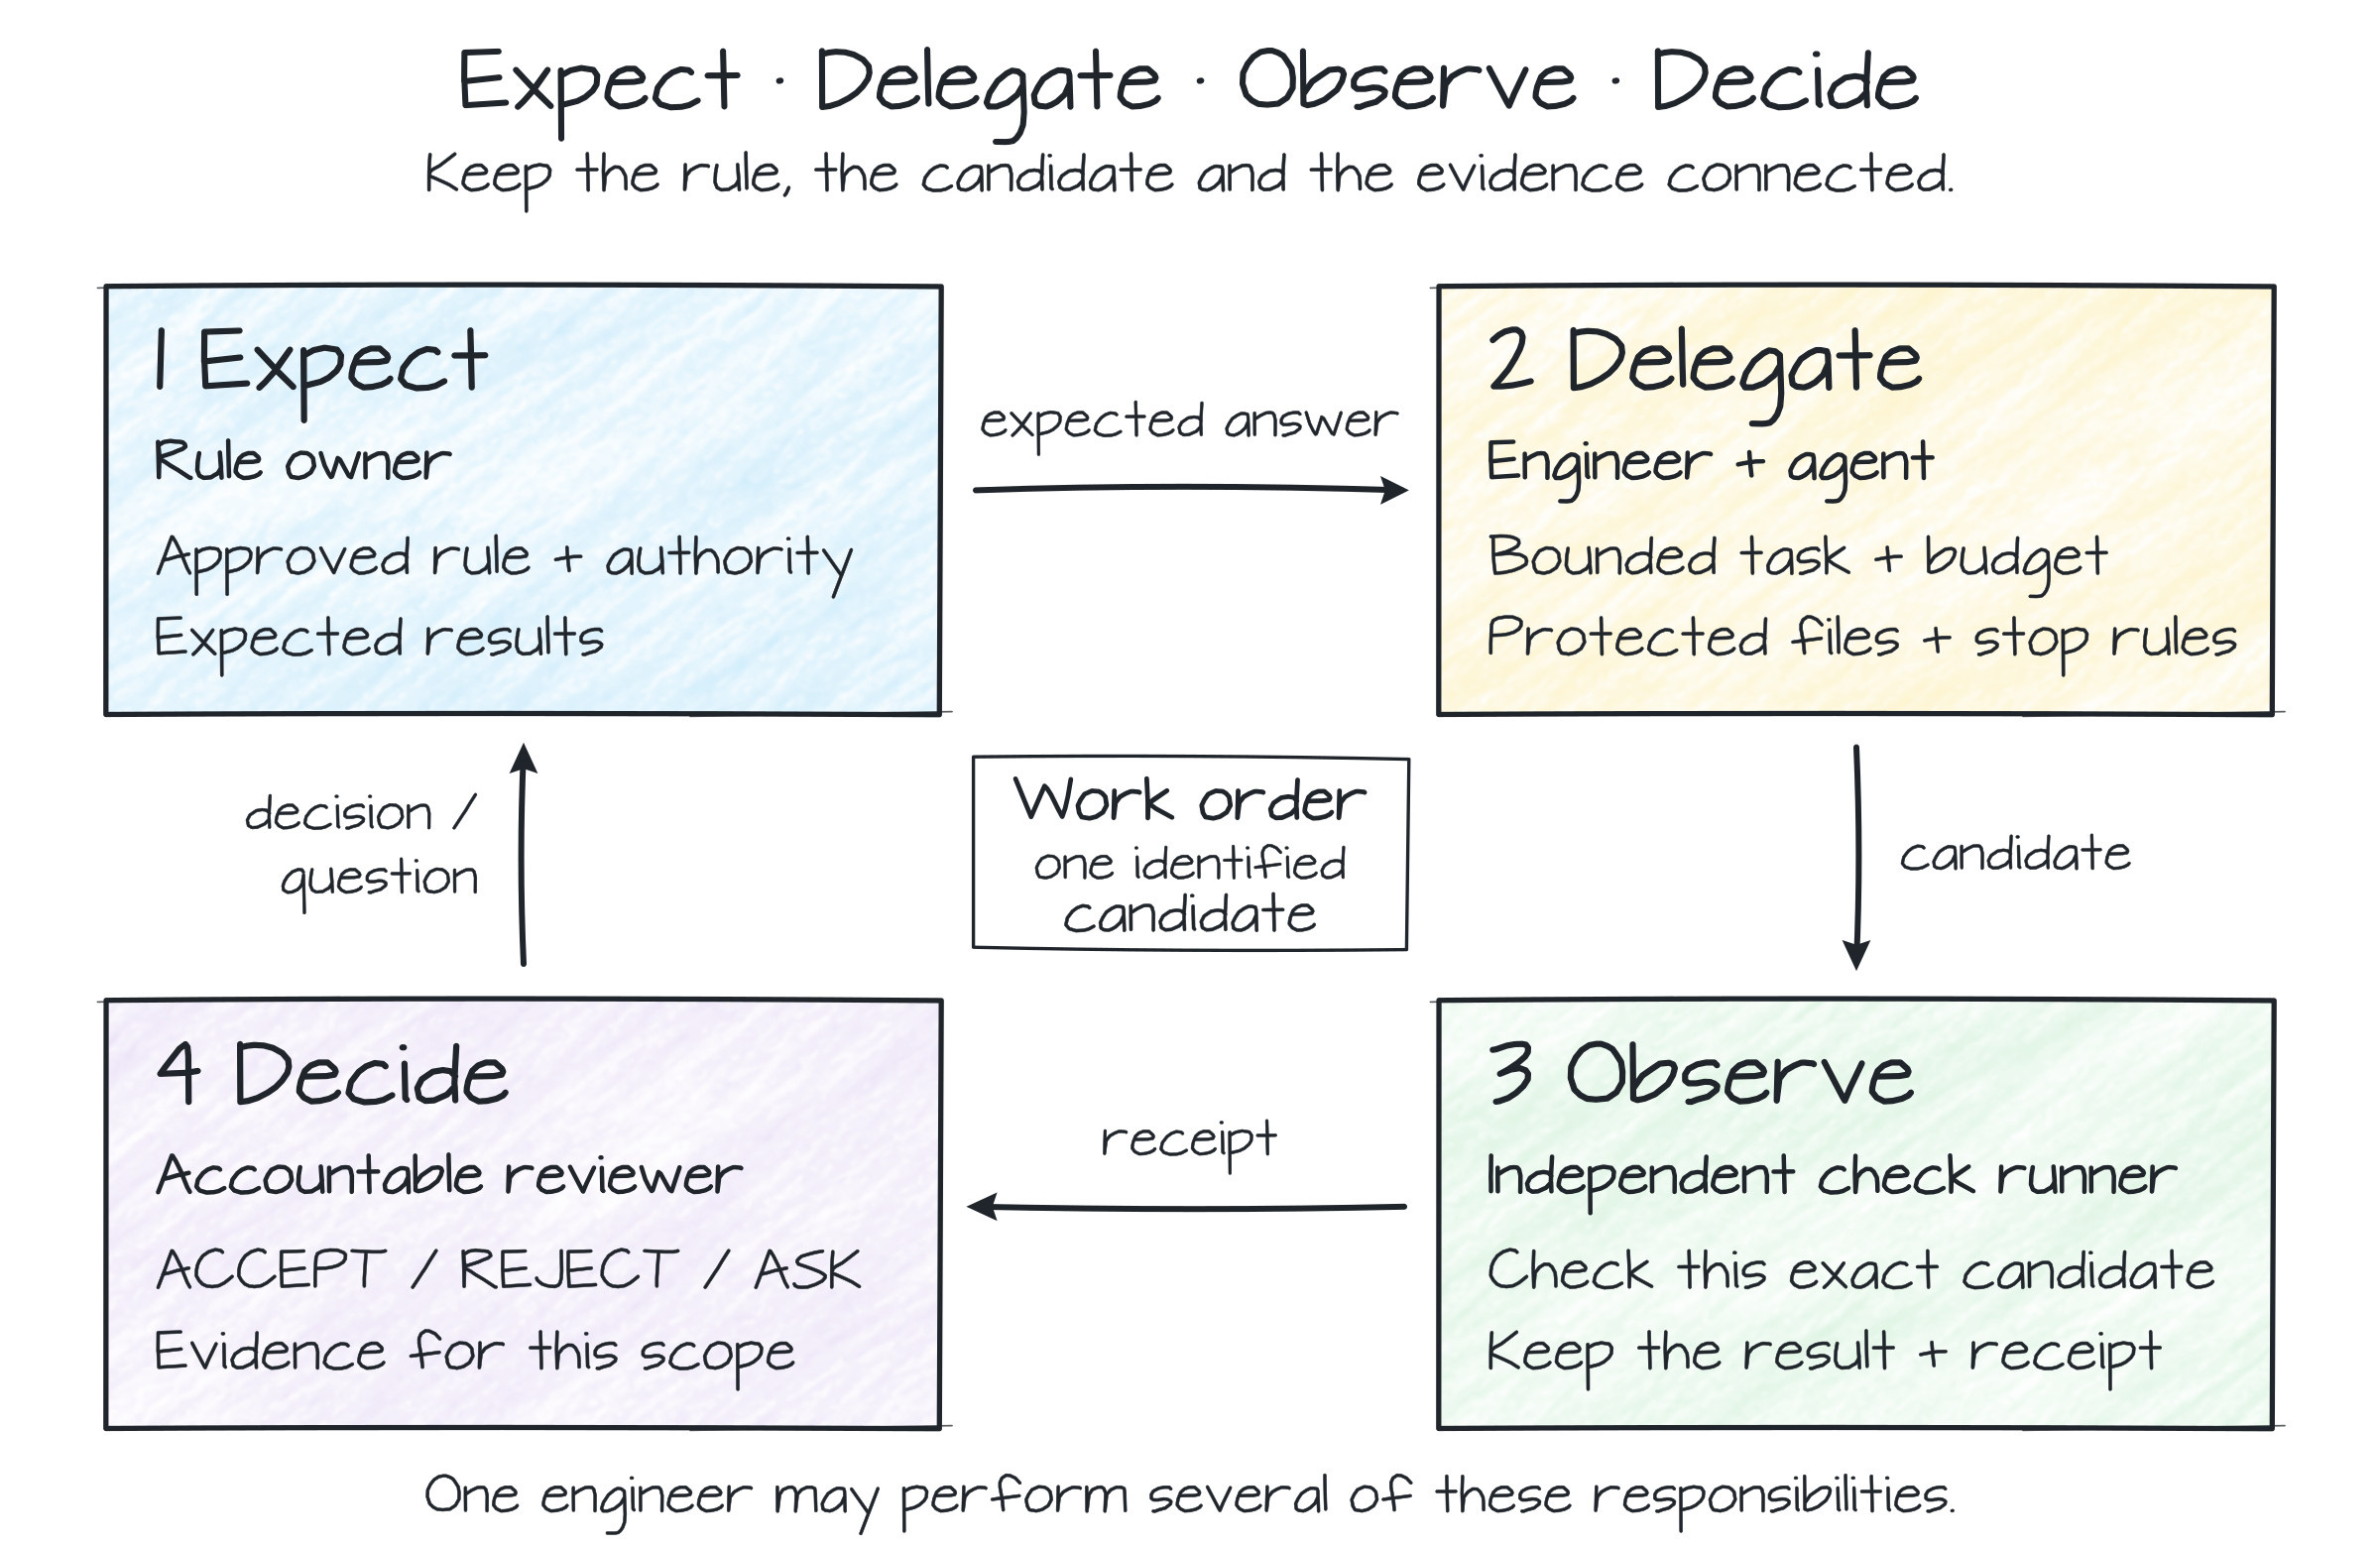
\includegraphics[width=\linewidth]{assets/edod.jpg}
\caption{EDOD connects an approved expectation to a bounded task, an observed candidate and an accountable decision. Hand-drawn adaptation of Figure~1.1 in Chapter~1.}
\end{figure}

\clearpage
\section{Seven green tests can leave the decisive case unchecked}

Here is the chapter's deliberately incomplete alternative. Reject the amount if it is \texttt{NaN} or at most zero. Keep the handling of malformed text, then compare the remaining amount with the threshold.

All seven core cases pass. Positive infinity survives that guard and reaches human review.

The policy already says the amount must be finite. An infinity check therefore tests a settled obligation. Its failure calls for a correction.

This is why test selection matters. \textbf{A useful check distinguishes the intended behaviour from a plausible wrong implementation.} Another ordinary positive amount would give us more green output while leaving this particular defect untouched.

The extended suite adds positive and negative infinity, another infinity spelling, signalling \texttt{NaN}, and a non-string caller. The last case checks a separate API promise: the function accepts strings and raises \texttt{TypeError} for another input type.

There is another trap. A broad exception handler can make all twelve methods pass while quietly converting an unexpected programming fault into an \emph{invalid amount} response.

The chapter addresses that promise with a different probe: inject a \texttt{RuntimeError} where decimal conversion happens and check that it remains visible. An invalid customer value and a defect in the program demand different responses.

More tests help when they challenge something that could still be wrong. Their total alone cannot tell us which promises have been examined.

\section{What the recorded agent actually did}

The weak guard is a teaching counterexample. The recorded repair in the chapter takes the fuller path.

An AI facilitator operates a fresh coding-agent session. The worker reads the contracts and starter, reproduces the failures, changes the router and checks its result. It validates the input type, catches the intended decimal-parsing exception, rejects nonfinite or nonpositive values, and preserves the original threshold comparison.

The recording uses a twelve-method development selection, larger than the seven-case core introduced earlier. All twelve pass after the repair. The worker also runs the injected-fault probe and checks two previously accepted text formats.

That is useful development evidence. The operator then invokes protected checks independently on the retained candidate. The chapter records a scoped conclusion: retain this v1 repair and stop the task.

For a reviewer, the important connection is between the rule, the check and the exact patch. If the code changes after the check, the earlier result does not automatically cover the new version. If the agent rewrites the expected answers to match its output, agreement has lost its value as a challenge.

\clearpage
\section{The decision is part of the engineering}

Chapter~1 gives the reviewer three decision labels.

\begin{itemize}
\item \textbf{ACCEPT}: this identified candidate meets the approved contract for the stated scope, with the required evidence and authority.
\item \textbf{REJECT}: an observation contradicts an obligation. Identify the contradiction and the correction it requires.
\item \textbf{ASK}: a consequential expectation or permission is missing. Identify the owner and the question.
\end{itemize}

The distinction becomes practical with inputs such as \texttt{1e3} and \texttt{4\_000}. Decimal parsing accepts them, and the current contract does not impose a narrower textual grammar. An agent tempted to \emph{clean up} those formats would be making a new product decision. The input-contract owner must settle that choice.

Infinity is different: the approved finite-amount rule already settles its rejection. We have enough authority to repair the implementation.

An interrupted check creates a third situation. If the runner cannot import the router, we have not observed its routing behaviour. Preserve the candidate, repair the checking setup and continue verification. A timeout can likewise leave useful code with checking still outstanding.

An accountable handoff tells the next person what exists, what actually ran and what remains unresolved. \emph{Candidate changed; verification incomplete} gives them a concrete next action.

This is the work I want engineers to recognise in agent-assisted development: define the outcome, direct the work, inspect the observations and control the acceptance decision. As implementation is delegated, those responsibilities need to stay visible.

\section{Take the next change further}

The first chapter gives you one small repair you can inspect from the approved rule to the retained result. The rest of \emph{Engineering Software with Agentic AI: Reliable Change with Coding Agents} takes that discipline into work with longer consequences.

The twelve chapters cover outcomes and specifications, context and tools, design, delegation, implementation, independent verification and release. Later chapters follow compatible history, diagnosis, learning and the whole cost of delivery.

Eight practical missions give those decisions continuity. A persistent workshop reservation grows through rules, migration, cancellation, integration and diagnosis. The Treasury course develops bounded provider work, preserved policy decisions and recovery. Each assignment carries earlier promises and stored state forward.

The book includes worked chapter decisions, mission solutions and an EDOD field card. Its \href{https://github.com/popoloni/esa_ai}{companion repository} provides material for following the examples and doing the practical work.

If you want a method you can use when an agent hands you a patch, start with Chapter~1 and carry it through the missions.

\textbf{\href{https://www.amazon.com/dp/B0HSPH86CG}{Buy Engineering Software with Agentic AI on Amazon.}}

The next time the agent says \emph{done}, you should be able to explain what you accepted---and point to the evidence.

\medskip
{\small\itshape Adapted by the author from Chapter~1, The first accountable change, in Engineering Software with Agentic AI, English review edition~5.6.1. Figures are redrawn from Figures~1.1 and~1.2.}
\end{document}
